%
% File: chap01.tex
% Author: Liam O'Shea
% Description: Introduction chapter where the boxing goes.
%
\let\textcircled=\pgftextcircled
\chapter{Background \& Research}
\label{chap:intro}

\initial{T}his chapter describes and explains boxing concepts which are important to understanding the goal of the project. It gives an overview of the types of punches a boxer must execute along with common errors associated with those. It also reviews relavant literature in areas covered by this thesis and explores the current cutting edge possibilities.

%=======
\section{Boxing Background}
\label{sec:sec01}

Boxing requires an incredible amount of co-ordination and timing as well as the ability to rapidly execute punches in a controlled and precise manner. Unlike professional boxing which is 12 x 3 minute rounds an amateur bout is 3 x 2 minute rounds which changes the dynamics of the contest. Amateur boxing relies on a points scoring system since there is often insufficient time for knockouts. therefore amateur boxers rely on the mastery of technique and proper form. Dropping you hand for a split second can open you up to an experienced boxer and could spell disaster.

As someone who has boxed for over 5 years and captain of the university boxing club I know how difficult it is to develop good technique and also how much time and experience is required from a coach to develop a new boxer. This one-on-one time is incredibly valuable, expensive and hard to come by. My aim is to be able to identify different types of punches and to offer some sort of quality metric as well as feedback advice. This will bring some much needed expert advice to a beginner who can practice in the comfort of their own home.

This could be especially useful for the university club since we get new waves of people every year who have never boxed before. 

Maybe note here how IT IS NOT A KINECT BOXING GAME.

\subsection{Motivation}
\label{subsec:subsec01}

Every year the Amateur boxing club taking in new members that are total beginners. We spend an enormous amount of time and effort helping them learn the basics and encourage people to practice at home. The problem is that it’s incredibly hard to spot your own faults. If it was possible to practice at home with the benefits of coaching it would bring massive improvements to their abilities. It could also be used as a platform think it would be a great way to introduce younger children to the sport since the Xbox/Kinect is incredibly popular and so it’s great from an inclusion perspective.
I also have several years of coaching experience to call upon and an array of local talent who would be able to offer advice if needed.

\section{Boxing Technique}
\label{sec:sec02}
For the scope of this project I am going to focus on the most common orthodox stance. There are tens of slight variations on each punch but I am going to focus on the core and important principles from which these can be built.

\subsection{Stance}
\label{subsec:subsec02}
The most fundamental building block of boxing is the stance, that is how you hold and position your body as well as the placement \& orientation of your feet. A good stance is crucial since it allows the boxer to be well balanced and light on their feet, allowing fast movement in any direction as well as the ability to quickly duck, weave, slip and bob and lay back to avoid punches. It is also crucial for offense since the power from punches come from the transfer of weight from one leg to another which requires a very specific twisting hip movement. Often beginners forget this crucial step and so I'm hoping to use this unique trait to help me judge quality later on. A successful stance should have the following characteristics:

- Left foot forward, right foot back with the feet slightly wider than shoulder width with a 45 degree angle twist.
- Right heel of the ground at all times with weight placed more on your back leg
- Slightly bent knees
- Chin tucked down
- Right hand on the right hand side of your chin, left hand should be a few inches in front of the left side of the face
- Elbows tucked in

\subsection{Punches}
\label{subsec:subsec03}
\paragraph{Jab}
The elbow should stay tucked in while the left fist extends with palms facing inwards before twisting your wrist at the last moment. The natural thing to do is extend the punch with palms facing down, unfortunately this immediately makes the elbow stick out which allows the opponent to easily see you are about to throw a punch (telegraphing) while opening up your body for a counter attack.
The punch should also finish so your arm is fully extended which helps to extend your reach and protect your chin before speedily returning it to the guard position.
Characteristic to target: Sticking out elbow

\paragraph{Cross}
The cross is designed as your heavy straight punch and as such is slower but more powerful. To get a \'snappy\' and powerful punch it is important to transfer your weight rapidly from your back leg to your front leg. Right hand. Characteristic: Rapid and specific hip movement

\paragraph{Hooks}
Your elbow should come out so it is shoulder height and your fist and shoulder should be at 90 degrees to each other. Again a rapid transfer of weight between hips is needed. {\bf Characteristic: Rapid and specific hip movement}

\paragraph{Uppercuts}
This required the fighter to crouch down into the squat position and throw a punch vertically upwards, with the aim of striking the opponent's chin.
Characteristics: Crouch, directly vertical punch, keeping guard close at all times.

%A figures matrix.
\begin{figure}[t!]
\centering
\begin{minipage}{3.3cm}
    \centering
    \subtop[]{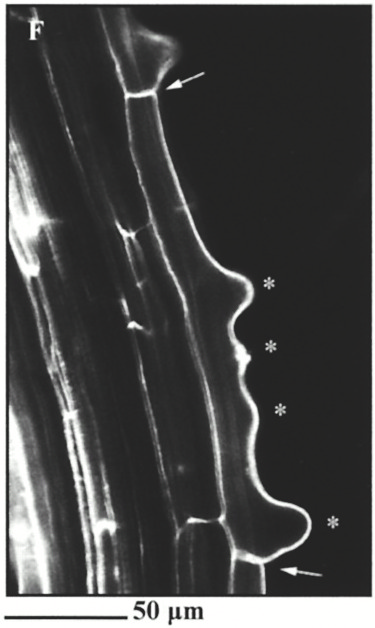
\includegraphics[height=0.28\textheight]{fig01/Nswellings}\label{sf:multiRH02a}}
\end{minipage}
\hspace{0.5cm}
\begin{minipage}{3.3cm}
    \centering
    \subtop[]{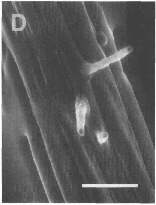
\includegraphics[height=0.27\textheight]{fig01/Mswellings}\label{sf:multiRH02b}}
\end{minipage}
\hspace{1.3cm}
\begin{minipage}{3.3cm}
    \centering
    \subtop[]{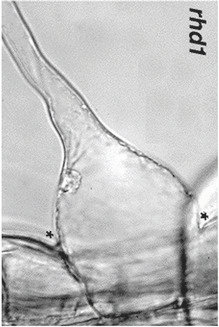
\includegraphics[height=0.27\textheight]{fig01/rhd1}\label{sf:multiRH02c}}
\end{minipage}
\\ \vspace{0.1cm}
\begin{minipage}{10cm}
    \centering
    \subtop[]{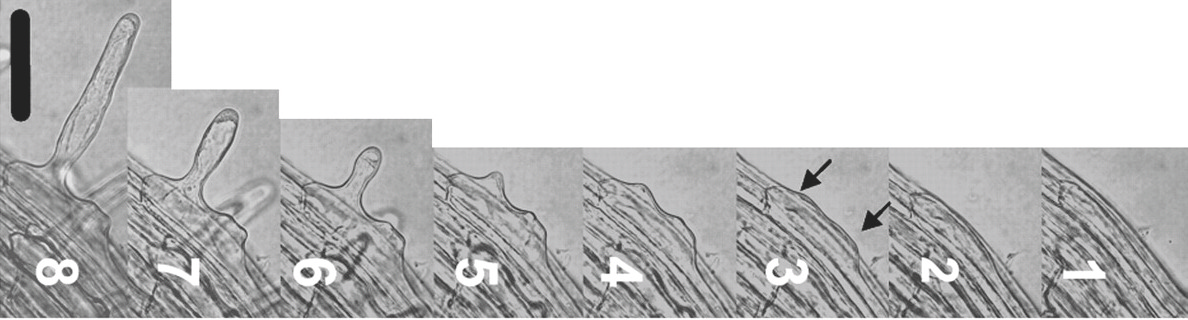
\includegraphics[height=0.145\textheight]{fig01/mutantrhd6}\label{sf:multiRH02d}}
\end{minipage}
\\ \vspace{0.1cm}
\begin{minipage}{10cm}
    \centering
    \subtop[]{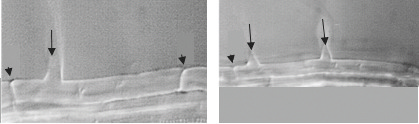
\includegraphics[height=0.16\textheight]{fig01/auxab}\label{sf:multiRH02e}}
\end{minipage}
\mycaption[Hair-forming mutant cells.]{(a) A mutant RH cell. Asterisks show multiple sites of RH initiation in a single root hair cell (indicated by the arrows). Figure reproduced from \cite{rigas01}. (b)~Hair-forming cell with three RH initiation locations. The bar represents $50\mu m$. Figure reproduced from \cite{massuci01}. (c) Large bump in mutant {\itshape rhd1}. Figure reproduced from \cite{griersonRH}. (d) Mutant overexpressing gene {\itshape ROP2}; from right-hand to left-hand, numbers indicate progressive snapshots at different times. RH initiation sites are indicated by the arrows. The bar represents $75\mu m$. Figure reproduced from~\cite{mjones01}. (e)~Mutants affected by auxin. On the left-hand side, RH site is farther away from the apical end (left arrow cap); on the right-hand side, multiple RH locations (arrows). Figure reproduced from~\cite{payne01}.}
\label{fig:multiRH02}
\end{figure}

% A single figure
\begin{figure}[t!]
	\centering
	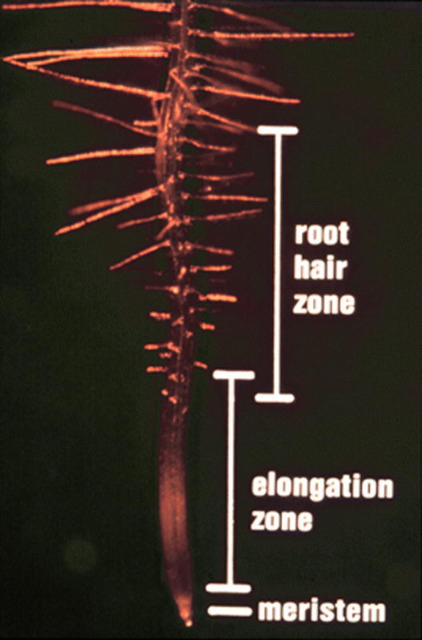
\includegraphics[height=0.35\textheight]{fig01/devepzones}
	\mycaption[Developmental zones of an Arabidopsis root.]{Developmental zones of an Arabidopsis root. Figure reproduced from \cite{griersonRH}.}
	\label{fig:RHP02}
\end{figure}

%=========================================================